\chapter{Comparación de los diseños y tipos de amortiguamiento}
\label{chap:comparacion}

\section{Comparación de las respuestas obtenidas}

La Figura~\ref{fig:escalon-comparacion} superpone las respuestas al escalón de ambos filtros y la
Tabla~\ref{tab:comparacion} resume sus parámetros. Si bien ambos diseños comparten la misma frecuencia de
corte, el comportamiento transitorio es claramente distinto: el filtro sobreamortiguado tarda unas cuatro
veces más en establecerse, pero su excursión por debajo del valor final es casi cinco veces menor que la
del filtro subamortiguado.

\begin{figure}[!ht]
  \centering
  \begin{tikzpicture}
  \begin{axis}[
    width=0.9\textwidth, height=0.5\textwidth,
    xlabel={$t$ [\unit{\milli\second}]}, ylabel={$v_o(t)$ [\unit{\volt}]},
    xmin=0, xmax=8, ymin=-0.3, ymax=1.05,
    grid=both, grid style={gray!30, dashed},
    legend pos=north east, legend cell align=left, legend style={font=\footnotesize},
    tick label style={font=\footnotesize},
    samples=400, domain=0:8, no marks,
  ]
    \addplot[blue, very thick] {1.07734*exp(-2.50072*x) - 0.07734*exp(-0.17953*x)};
    \addlegendentry{$Q = \num{0.25}$ ($\xi = 2$, sobreamortiguado)}
    \addplot[red!80!black, very thick]
      {exp(-1.77117*x)*(cos(deg(1.97975*x)) - 0.8946*sin(deg(1.97975*x)))};
    \addlegendentry{$Q = \num{0.75}$ ($\xi = \num{0.667}$, subamortiguado)}
    \addplot[gray, dashed] {0.02};
    \addlegendentry{banda de $\pm\qty{2}{\percent}$}
    \addplot[gray, dashed, forget plot] {-0.02};
  \end{axis}
\end{tikzpicture}

  \caption{Respuestas al escalón unitario para ambos valores de $Q$.}
  \label{fig:escalon-comparacion}
\end{figure}

\begin{table}[!ht]
  \centering
  \begin{tabular}{|l|c|c|}
    \hline
    Parámetro & $Q = \num{0.25}$ & $Q = \num{0.75}$ \\
    \hline
    Factor de amortiguamiento $\xi$                          & \num{2.000} & \num{0.667} \\
    Tipo de amortiguamiento                                   & sobreamortiguado & subamortiguado \\
    Raíces [\unit{\radian\per\second}]                        & $\num{-179.53}$ ; $\num{-2500.72}$
                                                              & $\num{-1771.17} \pm j\,\num{1979.75}$ \\
    Tiempo de caída (\qty{90}{\percent} a \qty{10}{\percent}) & \qty{0.70}{\milli\second}
                                                              & \qty{0.33}{\milli\second} \\
    Subpico máximo                                            & \qty{-4.8}{\percent} & \qty{-22.2}{\percent} \\
    Tiempo de establecimiento (\qty{2}{\percent})             & \qty{7.53}{\milli\second} & \qty{1.82}{\milli\second} \\
    Inductancia $L$                                           & \qty{37.31}{\milli\henry} & \qty{28.23}{\milli\henry} \\
    Capacidad $C$                                             & \qty{59.70}{\micro\farad} & \qty{5.02}{\micro\farad} \\
    \hline
  \end{tabular}
  \caption{Comparación de los parámetros de ambos diseños.}
  \label{tab:comparacion}
\end{table}

La diferencia en el comportamiento transitorio tiene su contraparte en la respuesta en frecuencia
(Figura~\ref{fig:bode-comparacion}). En el filtro sobreamortiguado los dos polos reales se encuentran muy
separados (\qty{28.6}{\hertz} y \qty{398}{\hertz}), de manera que entre ambas frecuencias la pendiente de
atenuación es de solo \qty{20}{\decibel} por década y la transición hacia la banda de rechazo es gradual.
En el filtro subamortiguado los polos complejos actúan en conjunto alrededor de $f_0 = \qty{422.8}{\hertz}$ y
la pendiente de \qty{40}{\decibel} por década se alcanza inmediatamente por debajo de la frecuencia de corte.
Como ejemplo, una señal de \qty{100}{\hertz} (dos octavas por debajo de $f_c$) se atenúa
\qty{12.6}{\decibel} con $Q = \num{0.25}$ y \qty{25.0}{\decibel} con $Q = \num{0.75}$. Para $Q = \num{0.75}$
el pico de resonancia es despreciable ($Q/\sqrt{1 - 1/(4Q^2)} = \num{1.006}$, equivalente a
\qty{0.05}{\decibel}), por lo que la banda de paso se mantiene prácticamente plana.

\begin{figure}[!ht]
  \centering
  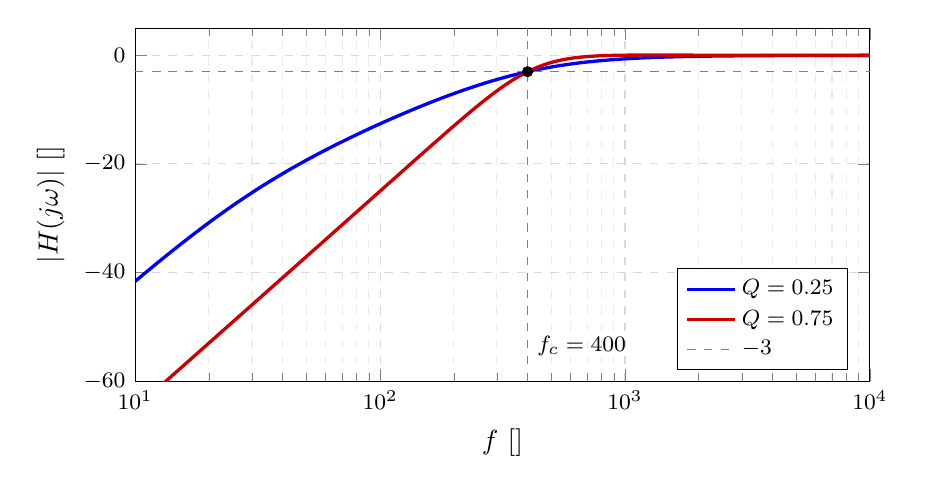
\begin{tikzpicture}
  \begin{semilogxaxis}[
    width=0.9\textwidth, height=0.5\textwidth,
    xlabel={$f$ [\unit{\hertz}]}, ylabel={$|H(j\omega)|$ [\unit{\decibel}]},
    xmin=10, xmax=10000, ymin=-60, ymax=5,
    grid=both, grid style={gray!30, dashed},
    minor grid style={gray!15, dashed},
    legend pos=south east, legend cell align=left, legend style={font=\footnotesize},
    tick label style={font=\footnotesize},
    samples=150, domain=10:10000, no marks,
  ]
    \addplot[blue, very thick]
      {20*log10((2*pi*x)^2 / sqrt((670.04^2 - (2*pi*x)^2)^2 + (670.04*2*pi*x/0.25)^2))};
    \addlegendentry{$Q = \num{0.25}$}
    \addplot[red!80!black, very thick]
      {20*log10((2*pi*x)^2 / sqrt((2656.40^2 - (2*pi*x)^2)^2 + (2656.40*2*pi*x/0.75)^2))};
    \addlegendentry{$Q = \num{0.75}$}
    \addplot[gray, dashed] {-3.01};
    \addlegendentry{$\qty{-3}{\decibel}$}
    \draw[dashed, gray] (axis cs:400,-60) -- (axis cs:400,5)
      node[pos=0.1, right, font=\footnotesize, black] {$f_c = \qty{400}{\hertz}$};
    \addplot[only marks, mark=*, mark size=1.8pt, black, forget plot] coordinates {(400,-3.01)};
  \end{semilogxaxis}
\end{tikzpicture}

  \caption{Módulo de la respuesta en frecuencia de ambos filtros.}
  \label{fig:bode-comparacion}
\end{figure}

\section{Ventajas de cada tipo de amortiguamiento}

\subsection{Sobreamortiguado ($\xi > 1$)}

\begin{itemize}
  \item La respuesta es no oscilatoria: no hay \emph{ringing} y el subpico es muy pequeño (en este diseño,
        del \qty{4.8}{\percent}), lo que resulta ventajoso cuando la señal filtrada alimenta etapas sensibles
        a excursiones de signo contrario (comparadores, detectores de nivel, etapas con limitación de
        excursión).
  \item El comportamiento es robusto frente a la tolerancia de los componentes: una variación de $L$, $C$ o
        de la resistencia de generador desplaza los polos sobre el eje real sin riesgo de que la respuesta
        se vuelva oscilatoria.
  \item La respuesta queda gobernada por una única constante de tiempo dominante, lo que simplifica su
        análisis y su predicción.
  \item Como contrapartida, el tiempo de establecimiento es largo y la transición entre la banda de paso y
        la de rechazo es poco selectiva; además, por ser $\omega_0$ mucho menor que $\omega_c$, se requieren
        componentes de mayor valor (en este caso un capacitor de \qty{59.70}{\micro\farad}).
\end{itemize}

\subsection{Críticamente amortiguado ($\xi = 1$)}

\begin{itemize}
  \item Corresponde a $Q = \num{0.5}$ y constituye el límite entre los dos casos anteriores: es la respuesta
        más rápida que puede obtenerse sin que aparezcan oscilaciones.
  \item Es la elección habitual cuando se busca minimizar el tiempo de establecimiento con la condición
        estricta de no sobrepasar el valor final.
  \item Su desventaja es que resulta un punto de diseño frágil: cualquier dispersión de componentes lo
        convierte en uno de los otros dos tipos.
\end{itemize}

\subsection{Subamortiguado ($\xi < 1$)}

\begin{itemize}
  \item Es el tipo de respuesta más rápida: en este diseño el tiempo de caída se reduce a la mitad y el
        tiempo de establecimiento a la cuarta parte respecto del caso sobreamortiguado.
  \item La respuesta en frecuencia es más selectiva: la pendiente de \qty{40}{\decibel} por década se
        alcanza inmediatamente por debajo de $f_c$ y la banda de paso es más plana, de modo que se filtran
        mejor las componentes cercanas a la frecuencia de corte.
  \item Al ser $\omega_0 \approx \omega_c$, los componentes resultan de menor valor (en este caso un
        capacitor de \qty{5.02}{\micro\farad}), lo que facilita su implementación con componentes no
        electrolíticos y de mejor tolerancia.
  \item La desventaja es la aparición de oscilaciones y de un subpico importante (\qty{22.2}{\percent}), que
        crece a medida que $Q$ aumenta; para valores de $Q$ superiores a $1/\sqrt{2}$ aparece además un pico
        de resonancia en la banda de paso que, para $Q = \num{0.75}$, todavía es despreciable.
\end{itemize}
